\section{Motivations}

\begin{frame}{$\mathrm{CO_2}$ Emission by Sector}

    Transportation sector is the second-largest contributor to $\mathrm{CO_2}$ emission.

    \vspace{9pt}

    \begin{figure}
        \centering
        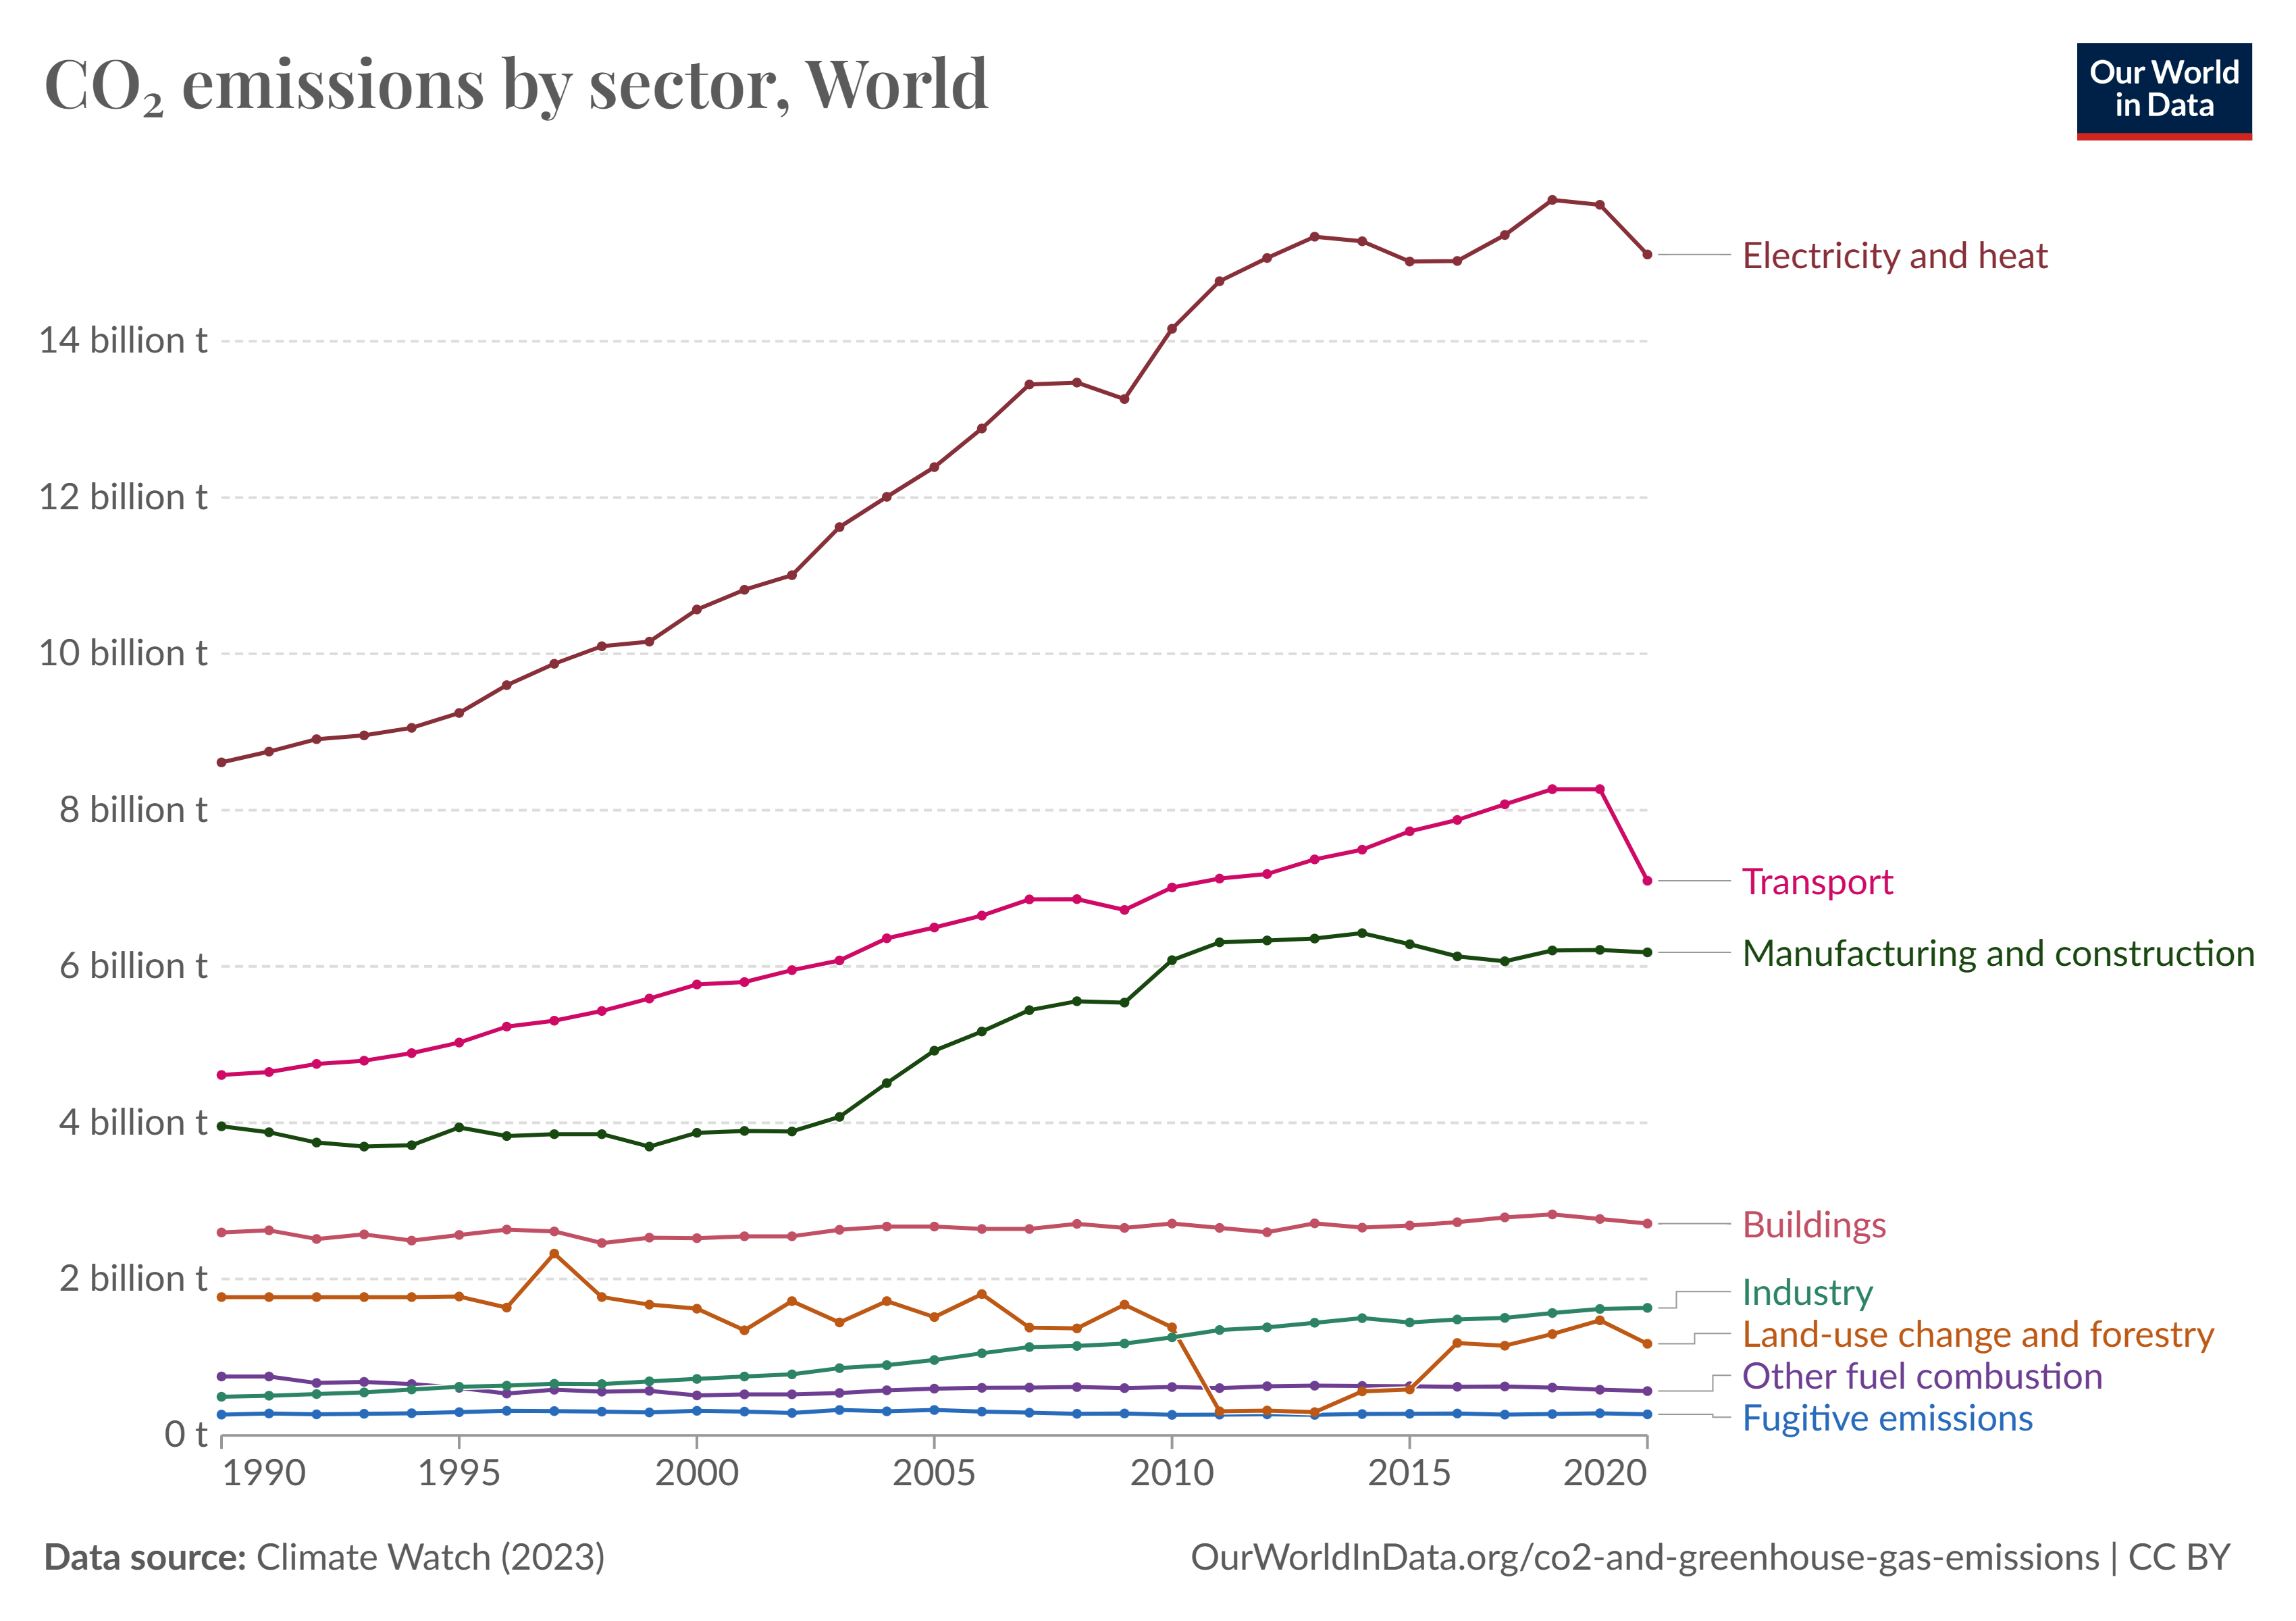
\includegraphics[width=0.8\textwidth]{img/co-emissions-by-sector.png}
        % \caption{$\mathrm{CO_2}$ Emission by sector}
    \end{figure}

\end{frame}



\begin{frame}{Alternative to traditional Fossil Fuel}

    Transportation sector has been looking for alternative fuels to reduce $\mathrm{CO_2}$ emission.

    \begin{itemize}
        \item \textbf{Electricity:} requires a large infrastructure to support the global demand
        \item \textbf{Methane:} worse than $\mathrm{CO_2}$ in terms of greenhouse effect (short-term)
        \item \textbf{Hydrogen:} difficult to store and transport
    \end{itemize}

\end{frame}



\begin{frame}{Ammonia as a Fuel}

    Researchers started looking at Ammonia as a potential alternative fuel.

    \vspace{9pt}

    \begin{columns}[c, onlytextwidth]

        \begin{column}{0.45\textwidth}

            \begin{figure}[H]
                \centering

                \LARGE
                \setchemfig{atom sep=5em, bond offset=5pt}
                \chemfig{\charge{90=\:}{N}(-[:210]H)(<[:290]H)(<:[:-15]H)}
                \normalsize

                \caption{Ammonia molecule ($\mathrm{NH_3}$)}

            \end{figure}

        \end{column}

        \begin{column}{0.55\textwidth}

            Advantages of Ammonia:

            \begin{itemize}
                \item No carbon content (zero $\mathrm{CO_2}$ emission)
                \item Long history of use in the chemical industry
                \item Possible use as hydrogen carrier
            \end{itemize}

        \end{column}

    \end{columns}

\end{frame}



\begin{frame}{Ammonia as a Fuel}

    \begin{columns}[c, onlytextwidth]

        \begin{column}{0.33\textwidth}

            \begin{figure}[H]
                \centering
                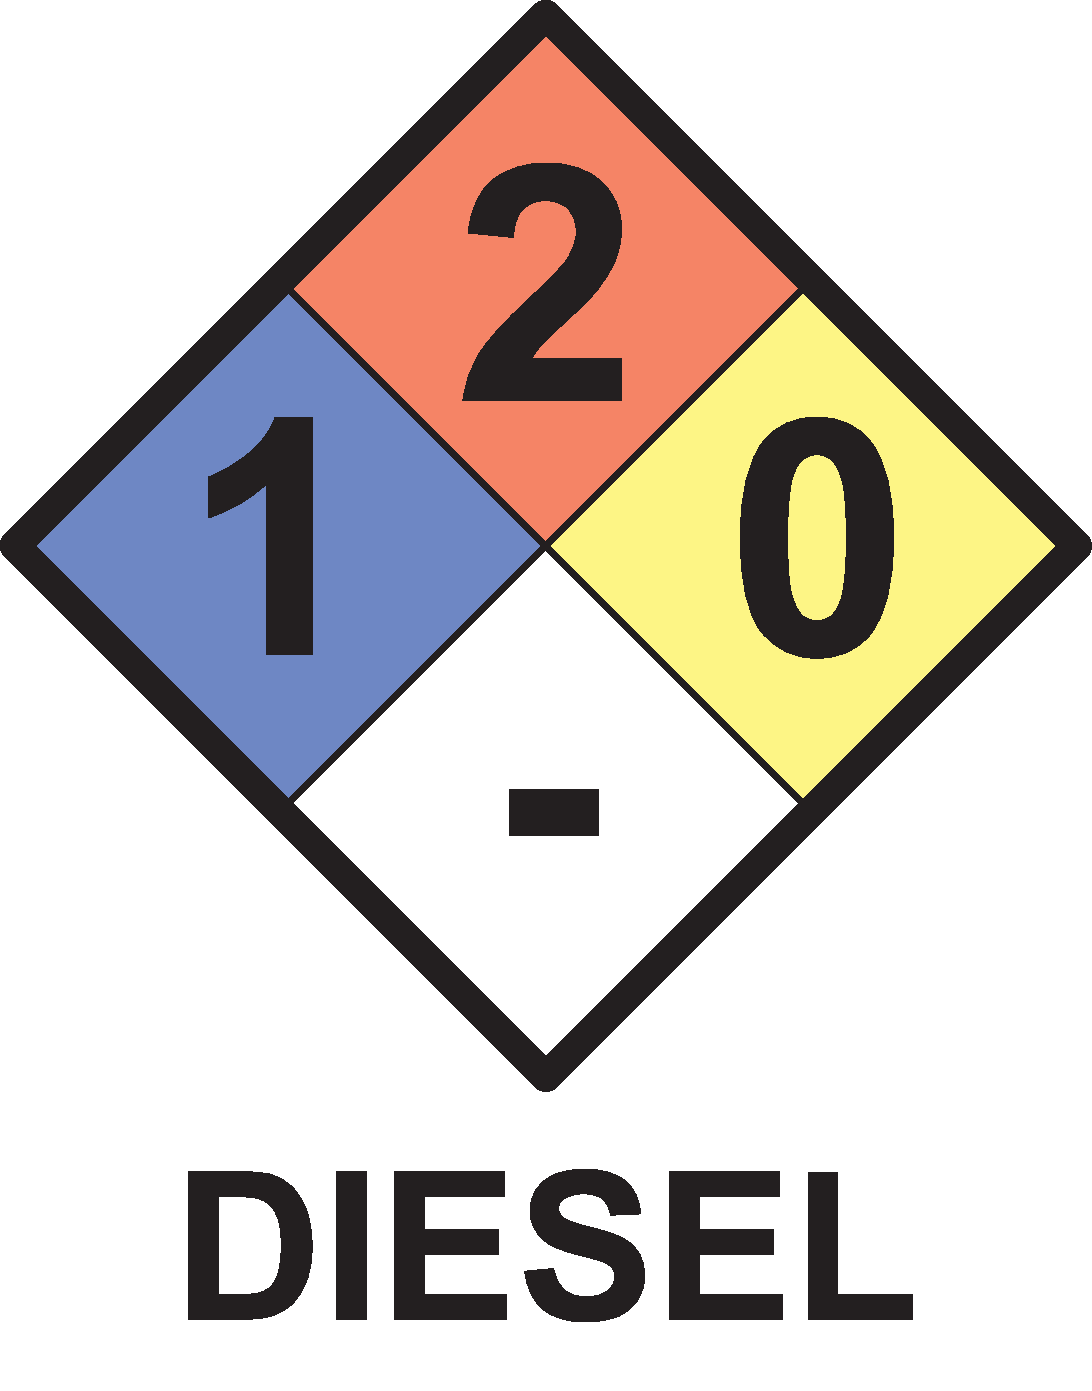
\includegraphics[width=0.5\textwidth]{pdf/nfpa-diesel.pdf}
            \end{figure}

        \end{column}

        \begin{column}{0.33\textwidth}

            \begin{figure}[H]
                \centering
                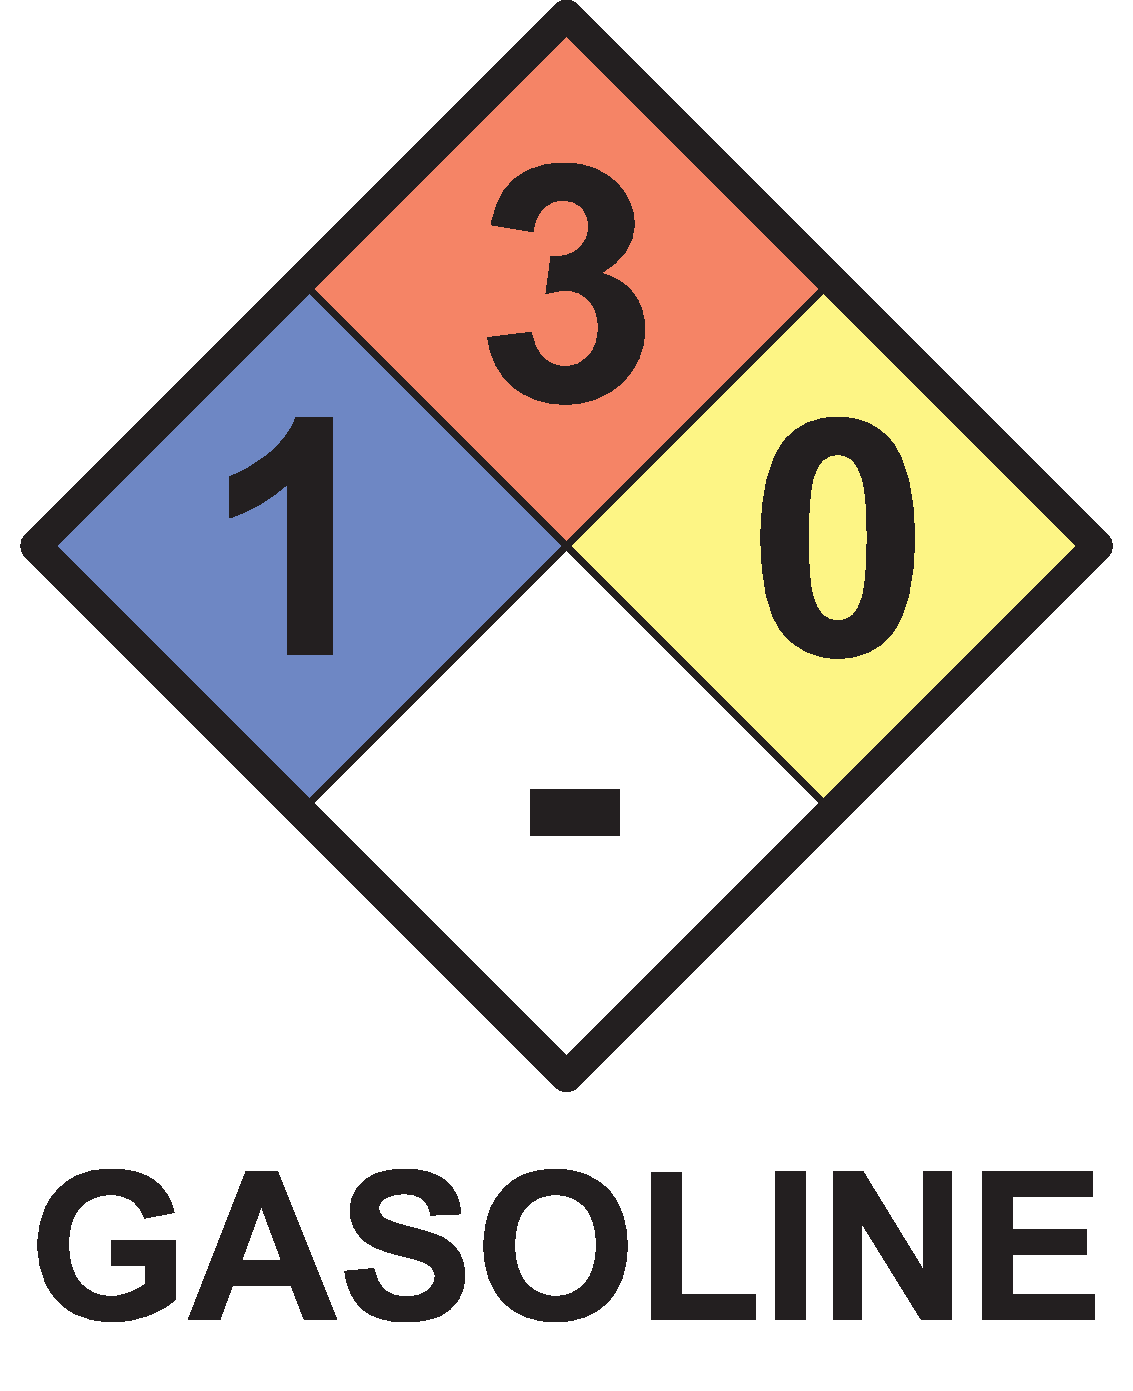
\includegraphics[width=0.5\textwidth]{pdf/nfpa-gasoline.pdf}
            \end{figure}

        \end{column}

        \begin{column}{0.33\textwidth}

            \begin{figure}[H]
                \centering
                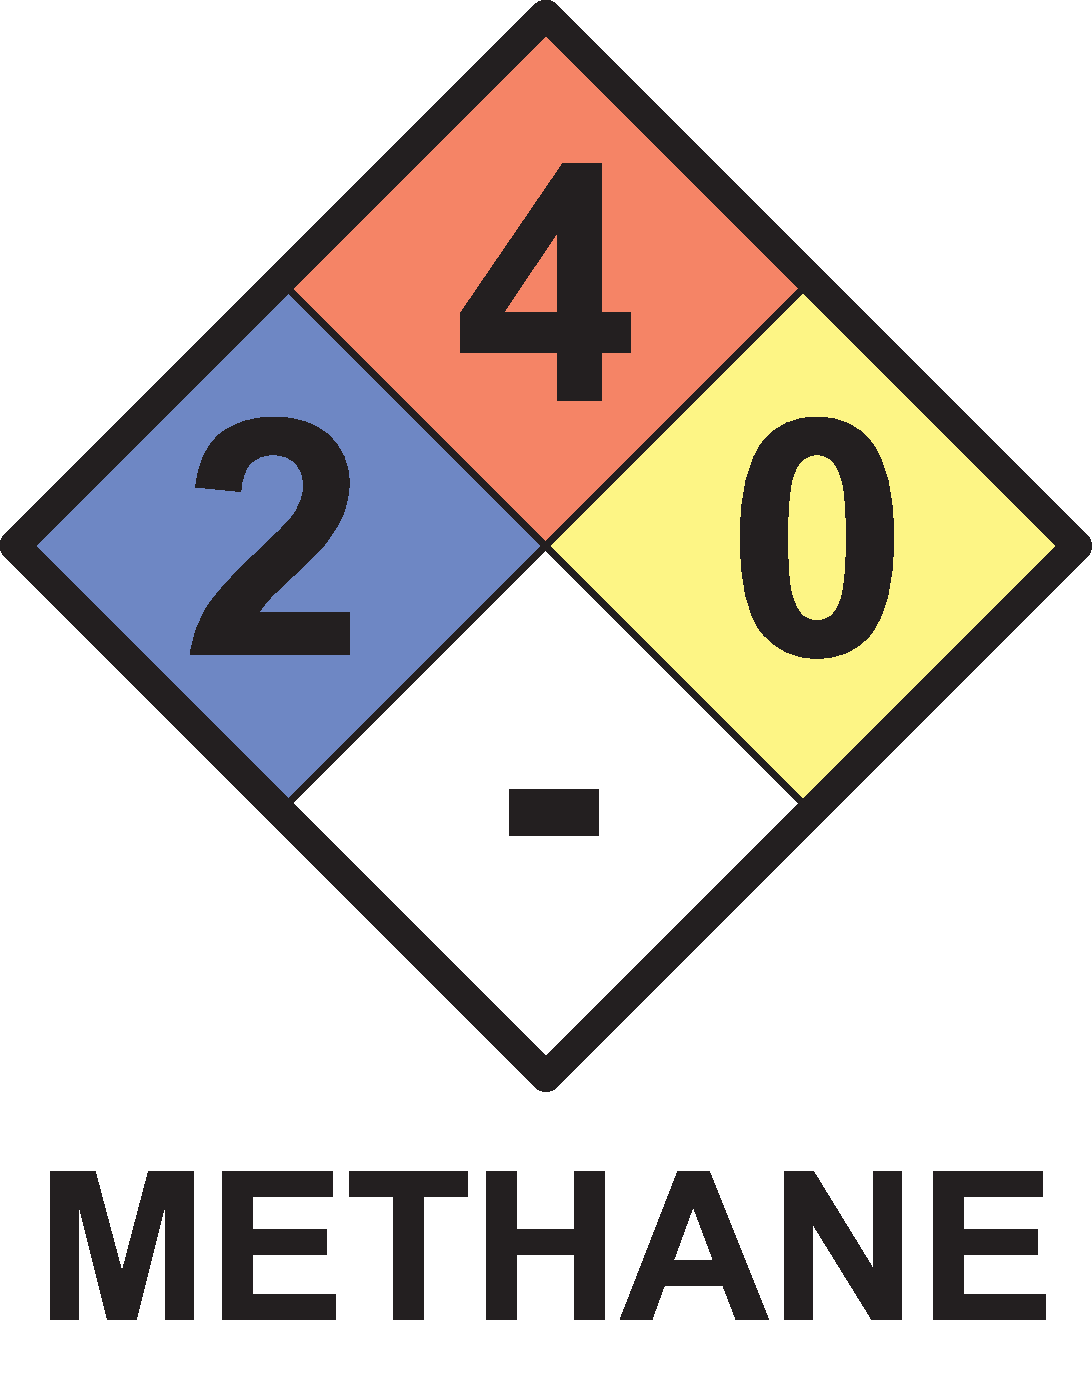
\includegraphics[width=0.5\textwidth]{pdf/nfpa-methane.pdf}
            \end{figure}

        \end{column}

    \end{columns}

    \begin{columns}[c, onlytextwidth]

        \begin{column}{0.4\textwidth}

            \begin{figure}[H]
                \centering
                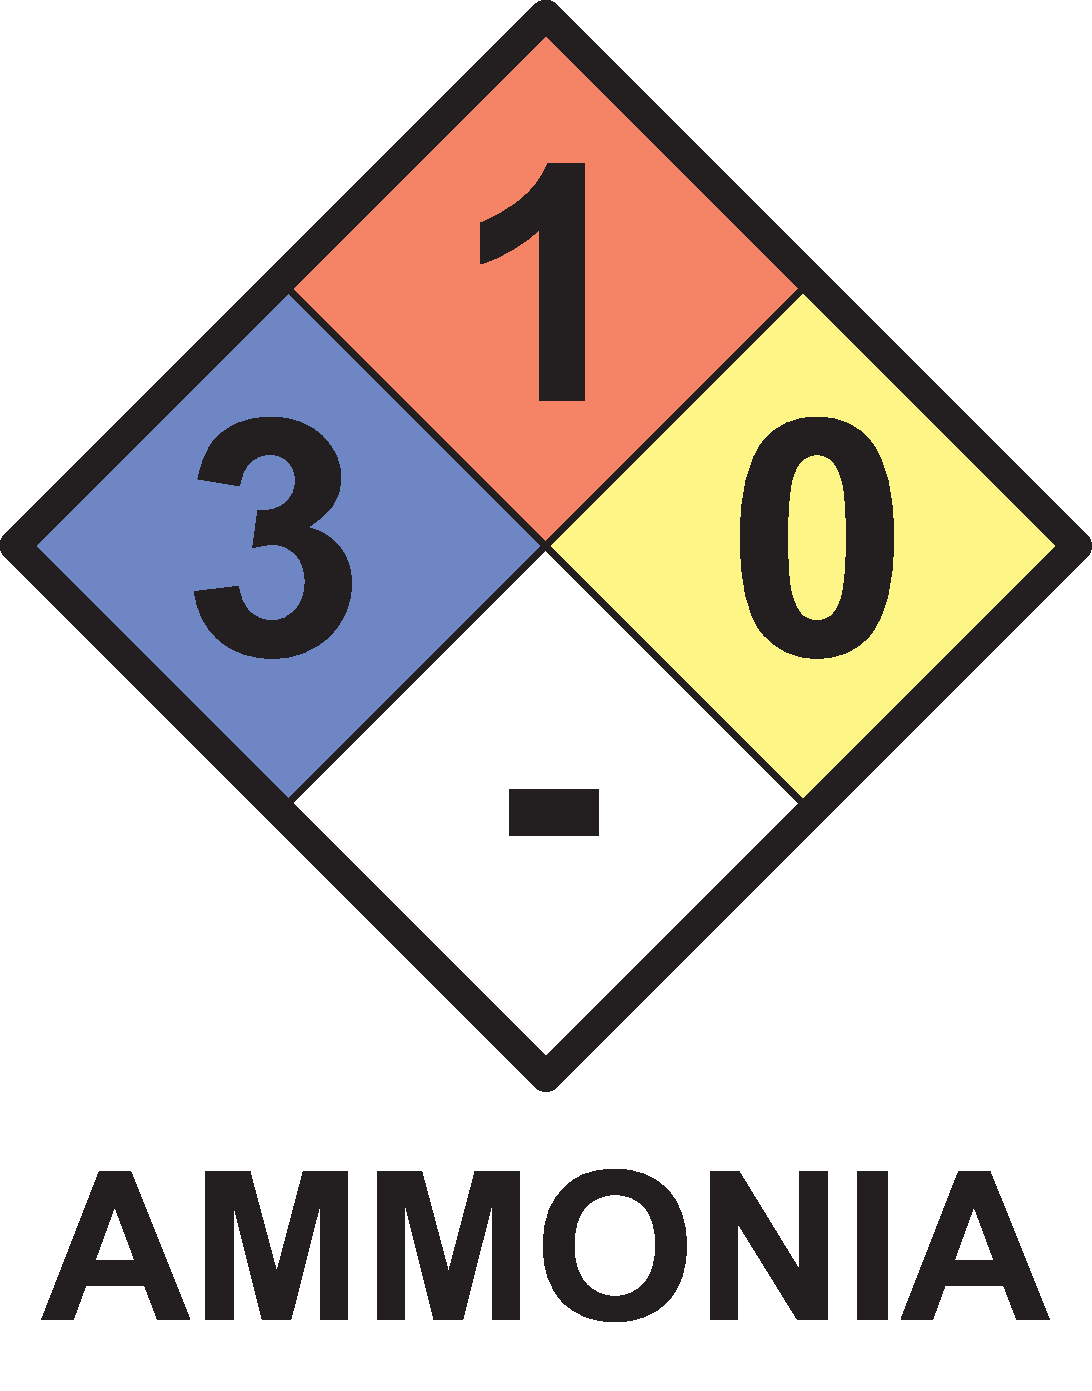
\includegraphics[width=0.5\textwidth]{pdf/nfpa-ammonia.pdf}
            \end{figure}

        \end{column}

        \begin{column}{0.6\textwidth}

            Disadvantages of Ammonia (also based on NFPAs\footnotemark[1]):

            \begin{itemize}
                \item Least flammable source, which also suggest \textbf{slow flame speed}
                \item Its combustion might produce \textbf{high $\mathrm{NO_x}$ emissions} if not properly controlled
                      % \item High ignition temperature
                      % Low flame velocity
                      % Slow chemical kinetics
            \end{itemize}

        \end{column}

    \end{columns}

    \footnotetext[1]{National Fire Protection Association 704: Standard System for the Identification of the Hazards of Materials for Emergency Response}

\end{frame}